\chapter{What next: Real-world results and opportunities for future work}
The famous Robert Feynman opened his 1965 Nobel Prize lecture by noting,
\begin{quote}
``\emph{We have a habit in writing articles published in scientific journals to make the work as finished as possible, to cover all the tracks, to not worry about the blind alleys or to describe how you had the wrong idea first, and so on. So there isn't any place to publish, in a dignified manner, what you actually did in order to get to do the work}...'' \cite{fey65}
\end{quote}
In this chapter, we include enough early commissioning results from the REIXS beamline to show that the design process produced a promising, feasible spectrometer-in-progress.  More importantly, however, we highlight the loose ends, blind alleys, and open questions that provide ongoing opportunities for future research.

\section{Spectrometer assembly, commissioning, and preliminary results}
After completing the optical design, we passed the requirements to a mechanical engineering firm to design the hardware that would position and interface all the spectrometer components.  Unfortunately, the firm shut down its operations immediately after rushing an early version of their design into production.  In addition to the grating manufacturing issues mentioned in Chapter 7, we had to correct many serious mechanical and system design flaws in the original assembly, which delayed the completion of the spectrometer by two years.  The issues are too numerous to detail completely, and outside the scope of this thesis, but we highlight some major examples:
\begin{itemize}
\item The detector vacuum chamber, with a mass of approximately 1200 kg, is lifted vertically into position by a ball screw drive and motor.  The ball screw was not equipped with a passive or active brake, so that loss of power to the lift motor would cause the chamber to instantly fall from the raised position (up to 1 meter).  If this had occurred, it could have destroyed the detector hardware.  More seriously, it posed a deadly hazard to users who could have been pinched or crushed if they were standing or reaching within certain regions of the machine.
\item The six-axis kinematic positioning system for the gratings did not have sufficient range to manoeuvre all six gratings into their operating positions.
\item The in-vacuum power supply and output signal cables for the detector were routed in a parallel bundle with unshielded stepper motor cables, causing electrical noise that swamped the actual detector signals.  The high voltage cables were required to apply up to four kilovolts, but were only rated for two kilovolts.
\item The original design required the detector's four-channel preamplifier to be sealed and placed in-vacuum beside the detector. However, the housing for the preamplifier could not maintain a positive seal.  Instead, we created a miniaturized re-design of the preamplifier using modern surface-mount components, which could be sealed using a standard UHV tube and flange.
\end{itemize}

We also spent a substantial amount of time determining how to align the optical components and process the detector images.  We developed processes and data acquisition software to
\begin{itemize}
\item focus the incident beam on the sample for maximum brightness,
\item align all optical components for proper focussing of the detector image, as a function of energy,
\item analyze the detector images, correcting for the curvature caused by the curved gratings and masking hot spots caused by light ionizing the detector housing,
\item correct for non-linearity in the detector position sensing, and
\item compute the scale for the spectrum energy axis based on the spectrometer geometry.
\end{itemize}

Refining these processes is an ongoing effort.  However, in the spring of 2012 all of this work culminated in forming the first useful emission spectra from the REIXS beamline.  In Figure \ref{impXES}, we show an example of the nitrogen K$\alpha$ emission line of hexagonal boron nitride (hBN), taken with the IMP grating.  From the observed count rate, we calculated that the spectrometer has an end-to-end throughput approximately four to six times higher than the Beamline 8.0.1 spectrometer\footnote{Unfortunately, the upstream beamline produces substantially less flux than Beamline 8.0.1, so the efficiency difference is practically negated for users.}, with comparable resolution.  This spectrum was developed in 20 minutes for 1892380 total counts.

\begin{figure}[htbp] %  figure placement: here, top, bottom, or page
   \centering
   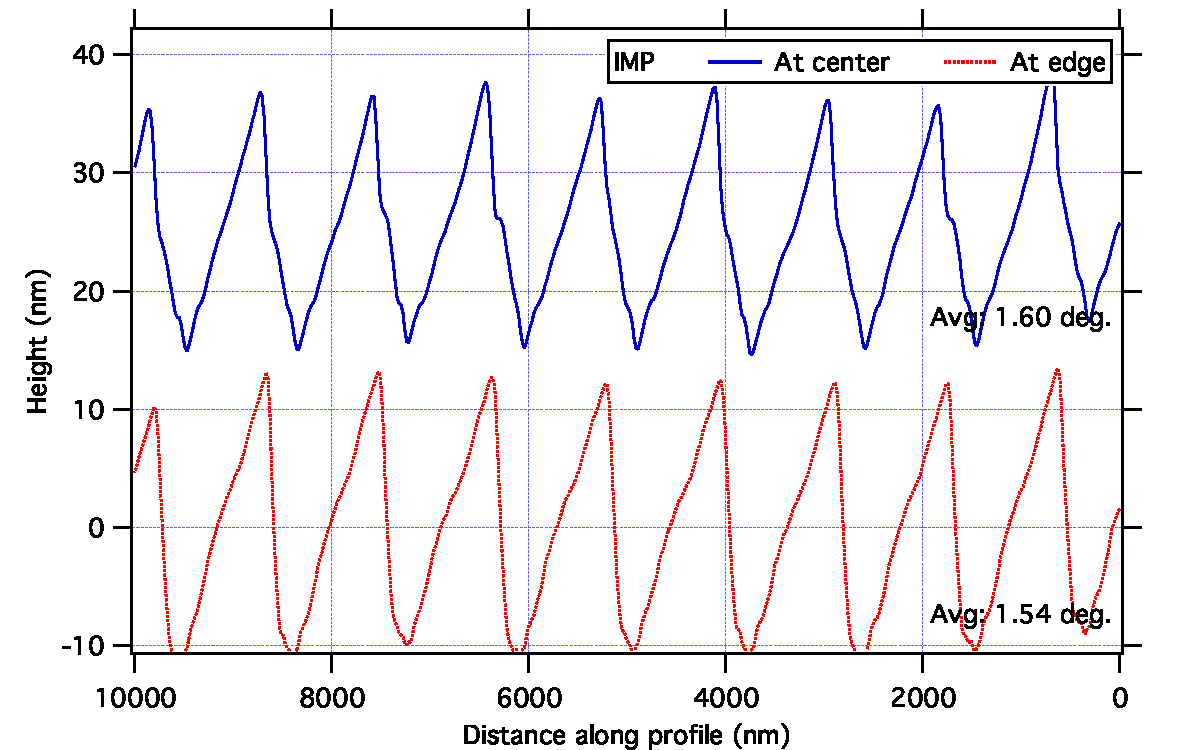
\includegraphics[scale=0.71]{Chapter6/IMP.pdf} 
   \caption{Nitrogen K$\alpha$ emission line of hexagonal boron nitride (hBN), taken using the IMP grating in 20 minutes.}
   \label{impXES}
\end{figure}

Figure \ref{megXES} shows the same spectrum measured using the medium energy grating.  The emission line covers more of the detector window, offering the possibility for higher resolution.  (The energy axis for this spectrum is in raw detector pixels instead of calibrated in eV.)

\begin{figure}[htbp] %  figure placement: here, top, bottom, or page
   \centering
   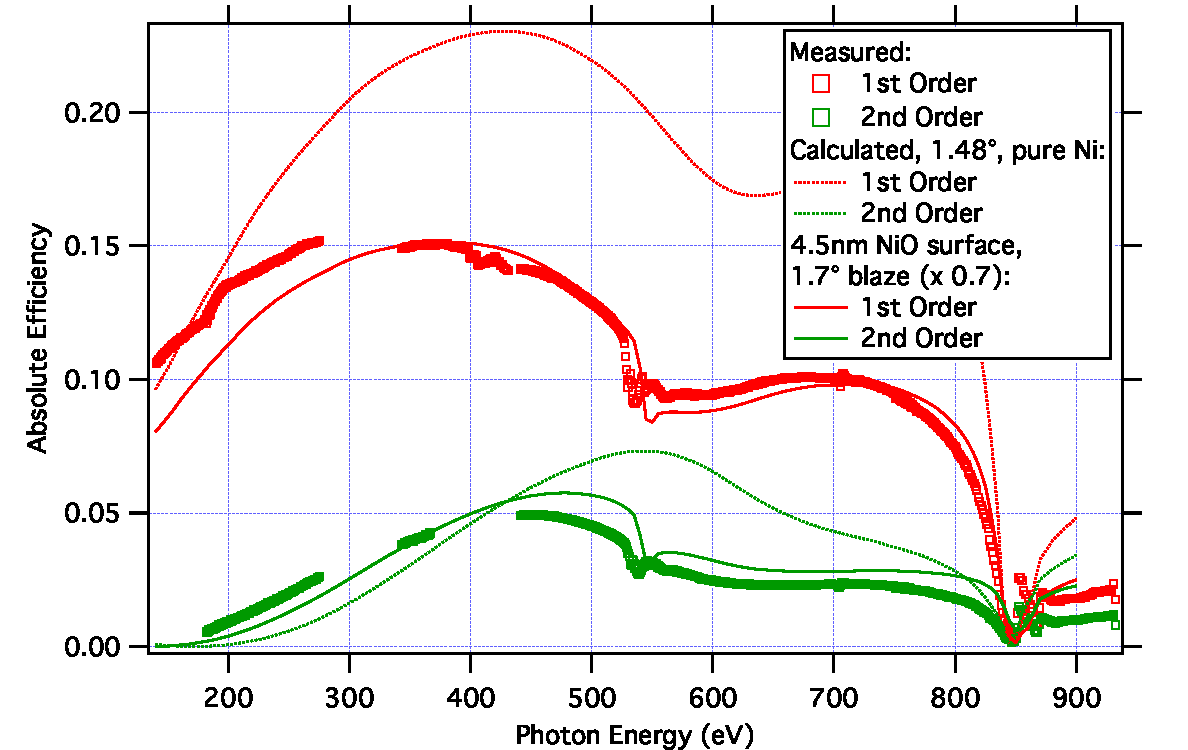
\includegraphics[scale=0.71]{Chapter6/MEG.pdf} 
   \caption{Nitrogen K$\alpha$ emission line of hexagonal boron nitride (hBN), taken using the MEG.  It offers the possibility for higher resolution than the IMP (Figure \ref{impXES}) at the expense of efficiency.  (The energy axis for this plot is not calibrated.)}
   \label{megXES}
\end{figure}

Using the HRMEG in third order should offer even higher resolution.  However, the low efficiency of the grating requires long count times to develop even poor statistics (Figure \ref{hrmegXES}).  Over this time, thermal expansion of the machine due to room temperature cycles causes the detector's central energy to shift, which reduces the resolution.\footnote{The temperature stabilization problem occurs with the other gratings as well, but becomes more significant at higher resolution and longer count times.} Work is still ongoing to focus the spectrometer for operation with the HRMEG, as well as stabilize the room temperature.

\begin{figure}[htbp] %  figure placement: here, top, bottom, or page
   \centering
   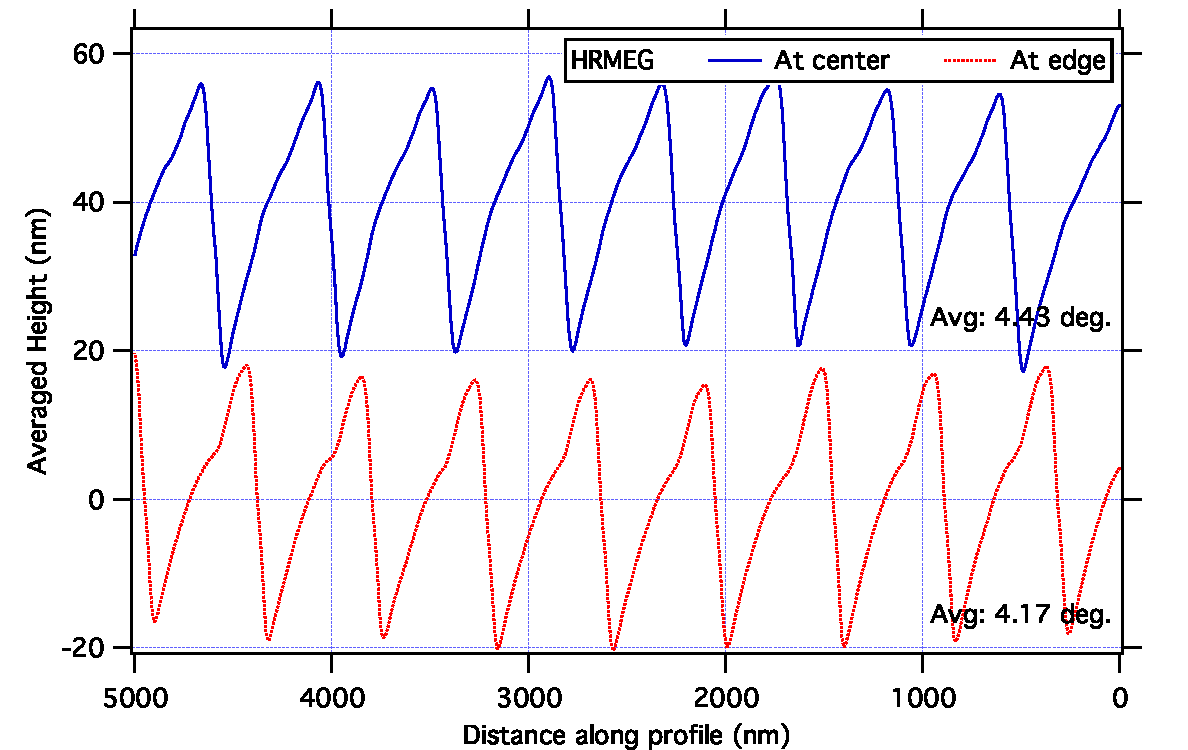
\includegraphics[scale=0.71]{Chapter6/HRMEG.pdf} 
   \caption{Nitrogen K$\alpha$ emission line of hexagonal boron nitride (hBN), taken using the HRMEG in third order.  The low count rate requires long count times; however, temperature shifts in the room cause the central detector energy to shift over this time, reducing the resolution.  Work is still ongoing to focus the spectrometer for operation with the HRMEG, as well as stabilize the room temperature.}
   \label{hrmegXES}
\end{figure}

\section{Future work: confirmation and extension of the fitting process}
We were surprised by the close agreement between the fitted and measured efficiency curves in Chapter 7.  The strong agreement between the fitted and AFM blaze angles suggests that we might actually be able to use efficiency measurements to characterize the profile and surface structure of gratings, especially when these are difficult to measure directly.  Several questions provide opportunities for future research:
\begin{enumerate}
\item Can the surface roughness and oxide thickness be measured experimentally to confirm the fitting predictions?
\item How many parameters can be fit simultaneously? Which parameters have overlapping and which have orthogonal effects on the shape of the efficiency spectra?
\item Without any prior knowledge of the nominal groove shape, could we predict the exact groove profile?
\end{enumerate}

Finally, we recognized in Chapter 7 that neither the Sinha nor Beckmann expressions provide a satisfactory description of surface roughness on gratings.  Both assume that the scattering due to roughness is independent of the diffraction order.  Additionally, the Beckmann expression is only valid near normal incidence, and the Sinha expression is only valid for roughness parameters much smaller than the wavelength.  We are still searching for a rigorous and general method to incorporate this into the calculated diffraction efficiencies.

\section{Future work: Efficiency calculation improvements and software-as-a-service}
One of our secondary goals was to encourage beamline designers to consider the grating efficiency at design time.  To support this goal, we would like to make grating calculation and optimization tools as complete and accessible as possible.

Within the existing software, we need to add the ability to compute TM efficiency.

Currently, we can optimize gratings using the solver to do single efficiency evaluations within a third-party or simple brute-force optimization tool.  However, it would be helpful to integrate a global optimizer into the software itself.  The optimizer should be able to accept an arbitrary set of grating parameters or ranges with constraints, and find the combination of parameters for maximum efficiency in the desired order.  Since optimization is resource-intensive, it should be able to run in parallel on high-performance computing platforms.

Finally, to make all of these tools as accessible as possible, we would like to build a web application to replace the \texttt{Gradif} interface shown in Chapter 4.  Instead of downloading, compiling, reading the documentation, and running the command-line software, users would have instant access to calculation and optimization services through their web browser.  By exploiting cloud computing resources such as Amazon's Elastic Cloud Compute (EC2) platform, results could be made available almost instantly, encouraging users to experiment and freely explore.